\section{From implemented mechanisms to an extensible core}
\label{section:from-a-working-core-to-an-extensible-sdk}

The route from these demonstrations to a reusable product is to expose the working core independently of this particular editor. Its organising unit is the object introduced above: an envelope carrying material, meaning and the grounds for using it. Such objects can be nested or linked without losing access to their detail. A result belongs to a calculation task, that task contributes to a comparison, and the comparison contributes to the project. Each level can expose a concise account while retaining a route to its detailed grounds. The \emph{altitude of a task} is the level at which its decision is being made: choosing a research direction, checking a calculation and editing a sentence need different observations of the same underlying work.

Figure~\ref{fig:dd-nested-work-sdk} follows this pattern through a parent task, a worker and an independent reviewer. The parent asks a bounded question and supplies the relevant context. The worker reads the necessary sources or runs the declared calculation, then returns a contribution with its evidence. The reviewer inspects that exact contribution. The parent consumes both the result and the review before deciding what belongs in the larger account. Context descends with the question, while observations and findings return with a known scope.

The current Work mechanism already distinguishes nesting from dependence. A containing goal contributes to the scope of its child tasks. A prerequisite relation specifies which completed contribution a later task relies on. Changing the parent goal can therefore change a child's scope, while changing an accepted prerequisite can require a consumer's acceptance to be reconsidered. This gives composed work an explicit basis at each level instead of treating the word \emph{done} as a timeless property. Historical completions remain recorded, while missing evidence about what they depended on remains visible.

\begin{figure}[htbp]
\centering
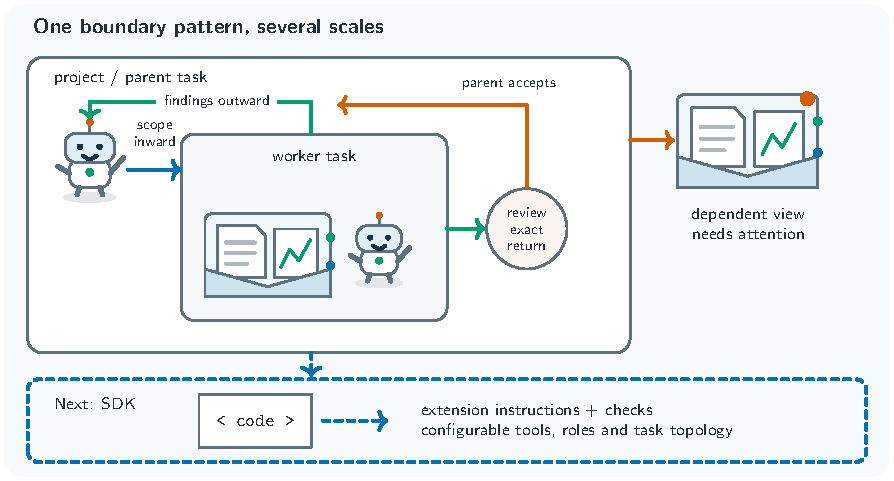
\includegraphics[width=\linewidth]{figures/robot-run-c4d4b3872a904ec0.result/dd-nested-work-sdk.pdf}
\caption{Composition across task altitudes. The parent sends a scoped question to a worker, receives an evidence-bearing contribution and consumes independent findings. Source, result and claim remain addressable within the child task. The amber marker on the neighbouring object shows where a changed input creates local review work. The dashed panel identifies the next SDK capabilities, using the same object and boundary vocabulary.}
\label{fig:dd-nested-work-sdk}
\end{figure}

Tools compose through the same discipline. One operation returns an identified result and the exact routes for inspecting or using it. The next operation consumes that result under its own conditions. A figure renderer, a claim-binding operation and a manuscript editor can therefore cooperate without sharing a hidden conversational memory. Their interfaces preserve the identity and meaning needed at the join.

The present system supplies the specialised objects, guarded tools, parent/worker/reviewer roles, bounded context and recorded acceptance used in this account. The next step is to package that working pattern as a standalone SDK. Its object templates should describe their states, allowed transitions, dependency effects and checks. Its extension instructions should travel with the code, so a developer can discover how a new capability fits rather than reconstructing the author's history.

A small extension makes the requirement tangible. An analysis module should declare its input types and revisions, output format, resource limits and failure behaviour. A result it produces should expose its interpretation and limitations, bind to the relevant claim and say which consumers need attention when an input changes. A new client should be able to inspect that result, propose a change and recover an interrupted operation through the same interfaces as the Writing App. The conformance examples should include successful use, a stale input, a repeated request and an attempted change outside the caller's authority.

This leads towards an operating environment for structured knowledge and agent work. An editor presents paragraphs and figures. A laboratory client presents samples and measurements. A research agent receives the objects needed for its task. A future frontend can let the author configure the topology and roles of a session network: which tasks run independently, which wait for evidence, who reviews them and where acceptance returns. The underlying contracts give those different interfaces a common meaning of identity, state and completion.

Source code already has a scoped place in this structure. The implementation exposes declared source inputs and human-granted development operations tied to a checkout, exact basis, permitted paths and checks. Retained source facts and their publication have separate owners. This is narrower than an autonomous ability to rewrite the running system. The SDK should make the relationship discoverable: a module's purpose, dependencies and checks should identify which behaviour a proposed change affects and which review may admit it. A useful increment can then increase the capacity available to build and inspect the next one without losing the boundary of the original permission.

The recursion matters because the same questions recur at each scale. What does this object retain? Which operation may change it? What does the change affect? What evidence makes the result usable? The SDK should make those questions answerable from its own interfaces and examples. A clean-environment test with an unfamiliar developer - one new result type, one second client, one interrupted operation recovered - would show whether the pattern has become a product that other people can extend.
